\section{Piezo Ramp Analysis (Piezo 2)}
\subsubsection*{Settings}

$f = 5.0$ Hz,  \\
Amplitude: 5.2 V,  \\
Offset: 0 V.  \\
Filename: \texttt{ALL0007.CSV}.   \\
Piezo No.; \texttt{2}  \\
Script: \texttt{overlayRamps.m} \\


In this, I try to understand the hystereis of the piezo. For this, I scanned several ramps and overlaid them.
I sorted them by High-Low and Low-High ramps. The results are shown in Figures~\ref{fig:fit_low} to \ref{fig:fit_low}.


\begin{figure}[H]
    \centering
    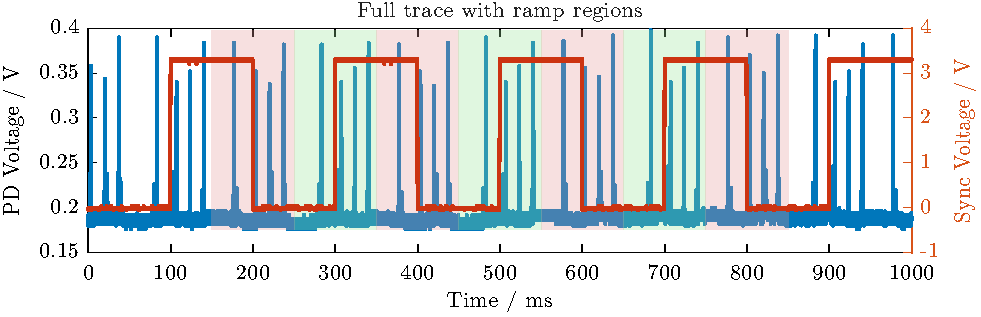
\includegraphics[width=\textwidth]{ManyRamp/ManyRamps.pdf}
    \caption{High-Low-Ramp: Red, Low-High-Ramp: Green}
\end{figure}

\begin{figure}[H]
    \centering
    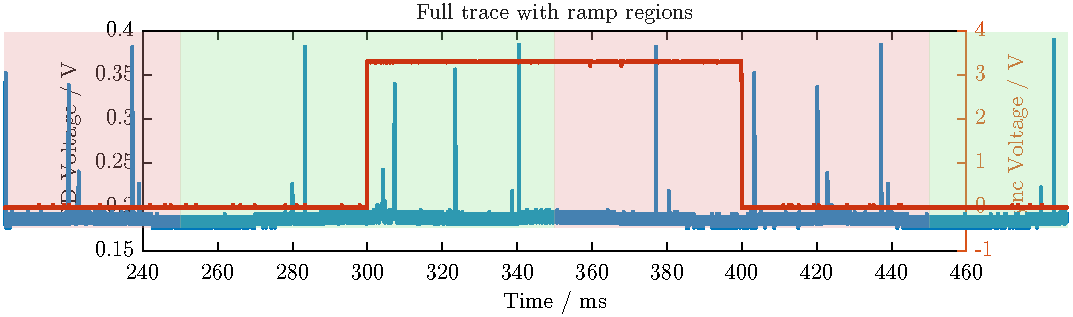
\includegraphics[width=\textwidth]{ManyRamp/Zoomed_Ramp.pdf}
    \caption{Zoom in section from the previous figure. It is worth mentioning that the peaks are not symmetrically spread around the turning point for the piezo. The turning point is at the border between a red and a green area.}
\end{figure}

\newpage

\begin{figure}[H]
    \centering
    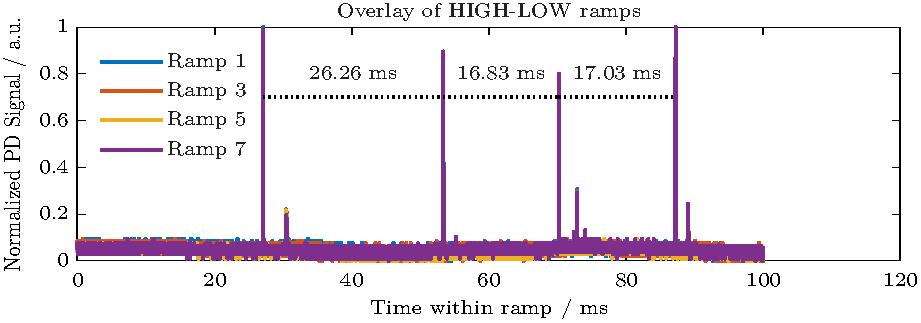
\includegraphics[width=\textwidth]{ManyRamp/HiLo.pdf}
    \caption{Here, I overlaid all the High-Low ramps and determined the average peak distance. It seems that it is not linear.}
\end{figure}

\begin{figure}[H]
    \centering
    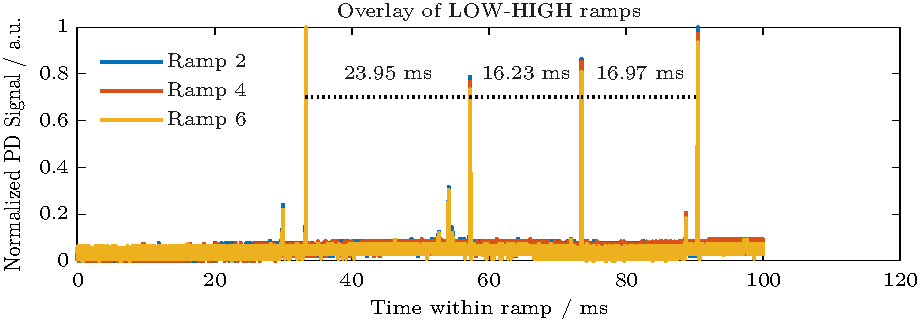
\includegraphics[width=\textwidth]{ManyRamp/LoHi.pdf}
    \caption{Same with this figure, but for the Low-High ramps.}
\end{figure}

It is super strange to me that the peak distances seem so arbitrary. 
You need to keep in mind that the piezo was moving in the \textbf{opposite} direction for each of the above figures, however, the distances do not seem to be mirror images of each other.
I would have expected that the distances are the same, just mirrored. But they are not.
When looking at the smaller surrounding peaks, it is obvious that the piezo changed direction (in the first figure, the smaller peaks are behind the large peak - in the second figure they are in front of them).
I do not have a good answer for this behavior. Perhaps, the FSR is not between these two similarly sized peaks, but between two different ones.
If this were true, the finesse may perhaps be up to three times higher.
\newpage
\subsection{Other Piezo (Piezo 1)}
The switch to the second piezo did not change the signal noticeably.
Same settings as before, just a different piezo. File used \texttt{ALL0008.CSV}, Piezo No. \texttt{1}.
\begin{figure}[H]
    \centering
    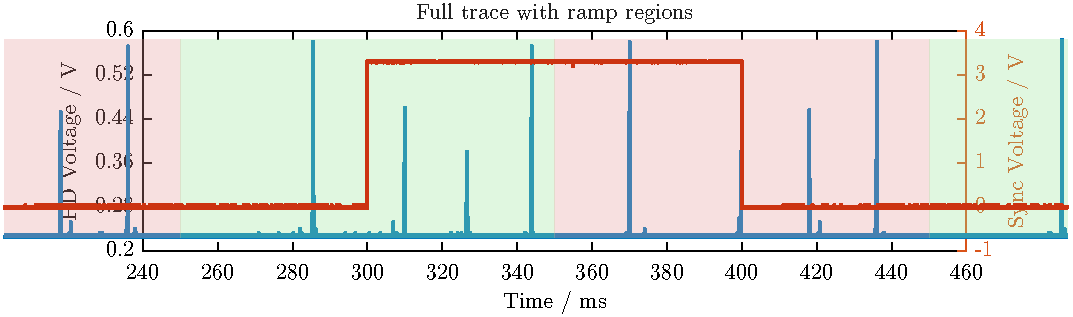
\includegraphics[width=\textwidth]{ManyRamp/Zoomed_Ramp2.pdf}
    \caption{Same as before, but with a different piezo.}
\end{figure}


\begin{figure}[H]
    \centering
    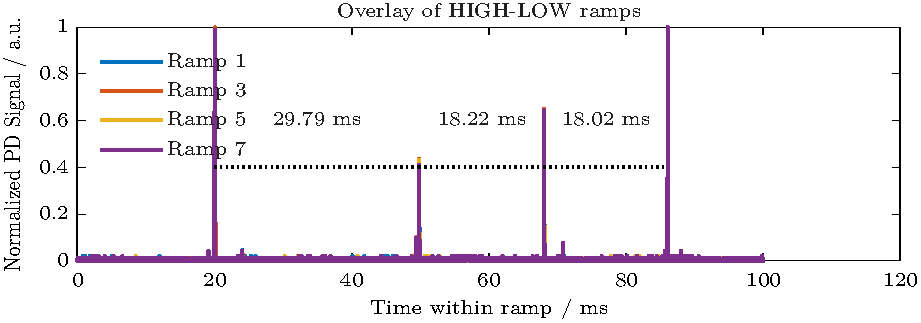
\includegraphics[width=\textwidth]{ManyRamp/HiLo2.pdf}
    \caption{Same as before, but with a different piezo.}
\end{figure}

\begin{figure}[H]
    \centering
    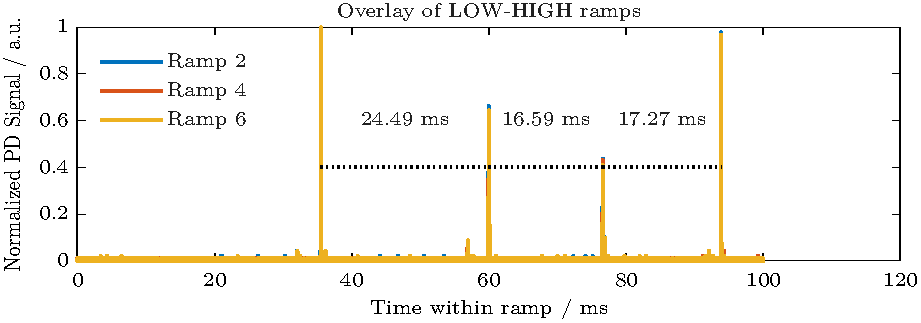
\includegraphics[width=\textwidth]{ManyRamp/LoHi2.pdf}
    \caption{Same as before, but with a different piezo.}
\end{figure}
